% !TeX spellcheck = de_DE
\documentclass[.../Dokumentation.tex]{subfiles}
\begin{document}
    \subsection{Hardware}\label{sec-ita4-hardware}
        \subsubsection*{Visualisierung}
    %Platine, LED Streifen, Autostart %
    Der Programmcode und die benötigte Hardware für die Visualisierung funktionieren bereits, trotzdem müssen noch kleine Optimierungen vorgenommen werden. Zuerst wird die Funktionsweise des LED-Streifens überarbeitet. Zuvor haben alle LEDs dieselbe Farbe angezeigt, welche sich aus Rot und Grün zusammensetzt. Die Farbe Grün ist viel dominanter, sodass die LEDs auch bei mittlerer Verschmutzung noch die Farbe grün anzeigen. Erst bei starker Verschmutzung färben sie sich orange und danach rot. Mit der neuen Implementierung zeigen die LEDs unterschiedliche Werte an. Je nach Verschmutzungsgrad färbt sich ein Teil der LEDs rot (\autoref{fig-hardware-tree-half-ref}). Ist die maximale Verschmutzung erreicht, sind alle LEDs rot. Hierdurch wird die gesamte Verschmutzung eindeutig dargestellt.
    \begin{figure}[H]
    	\begin{center}
    		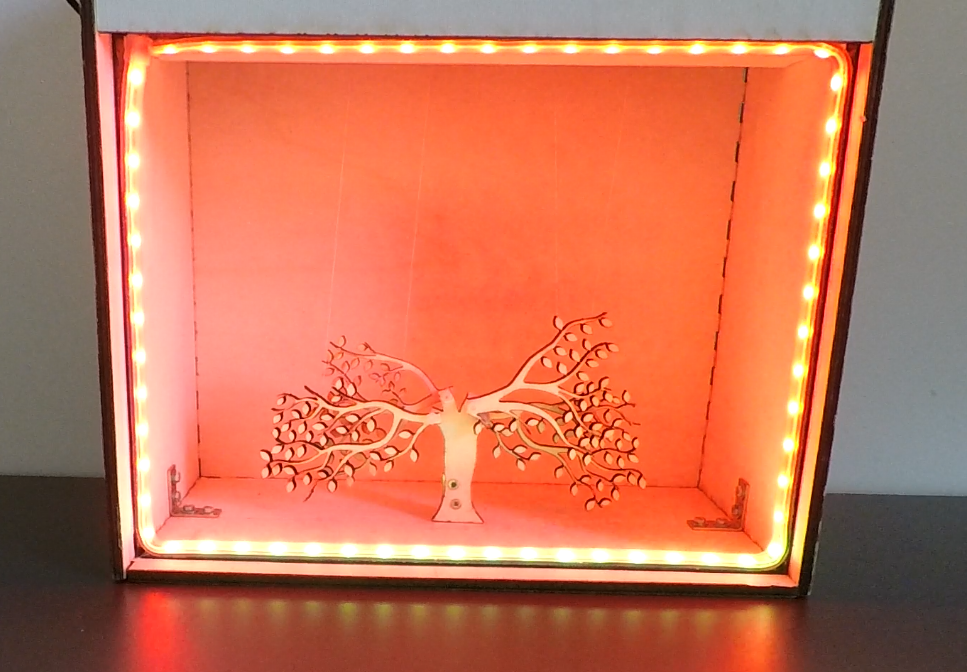
\includegraphics[
    		width=0.5\linewidth,
    		]{imgs/tree_half_red.PNG}
    		\caption{Visualisierung mit neuer LED-Stripe Implementierung}
    		\label{fig-hardware-tree-half-ref}
    	\end{center}
    \end{figure}
	\noindent
    Im nächsten Schritt wird noch eine Platine für den Raspberry Pi erstellt. Diese kann wie ein Shield auf die Pins gesteckt werden und die Servo Motoren sowie der LED-Streifen können direkt angeschlossen werden. Dies reduziert die Anzahl an benötigten Kabeln und erhöht die Übersichtlichkeit.\\
    Zuletzt wird die Konfiguration des Raspberry Pi überarbeitet. Der Flask-Webserver soll automatisch mit jedem hochfahren des Systems gestartet werden. Somit muss, wie auch bei den Fahrzeugen, nur die Stromversorgung hergestellt werden, um den Prototypen zu benutzen.
        
    \subsubsection*{Fahrzeug}
    Für die voll funktionsfähige und getestete Schaltung muss eine Prototyp Platine erstellt werden. Die Basisplatine hat dieselbe Größe wie der Arduino. Somit kann die fertige Platine wie ein Shield auf den Arduino gesteckt werden und verbraucht wenig Platz. Allerdings muss das Layout wegen der begrenzten Größe vorher geplant werden. Eine Skizze hierfür ist in Abbildung \ref{fig-hardware-car-pcb-plan} dargestellt. 
    \begin{figure}[H]
    	\begin{center}
    		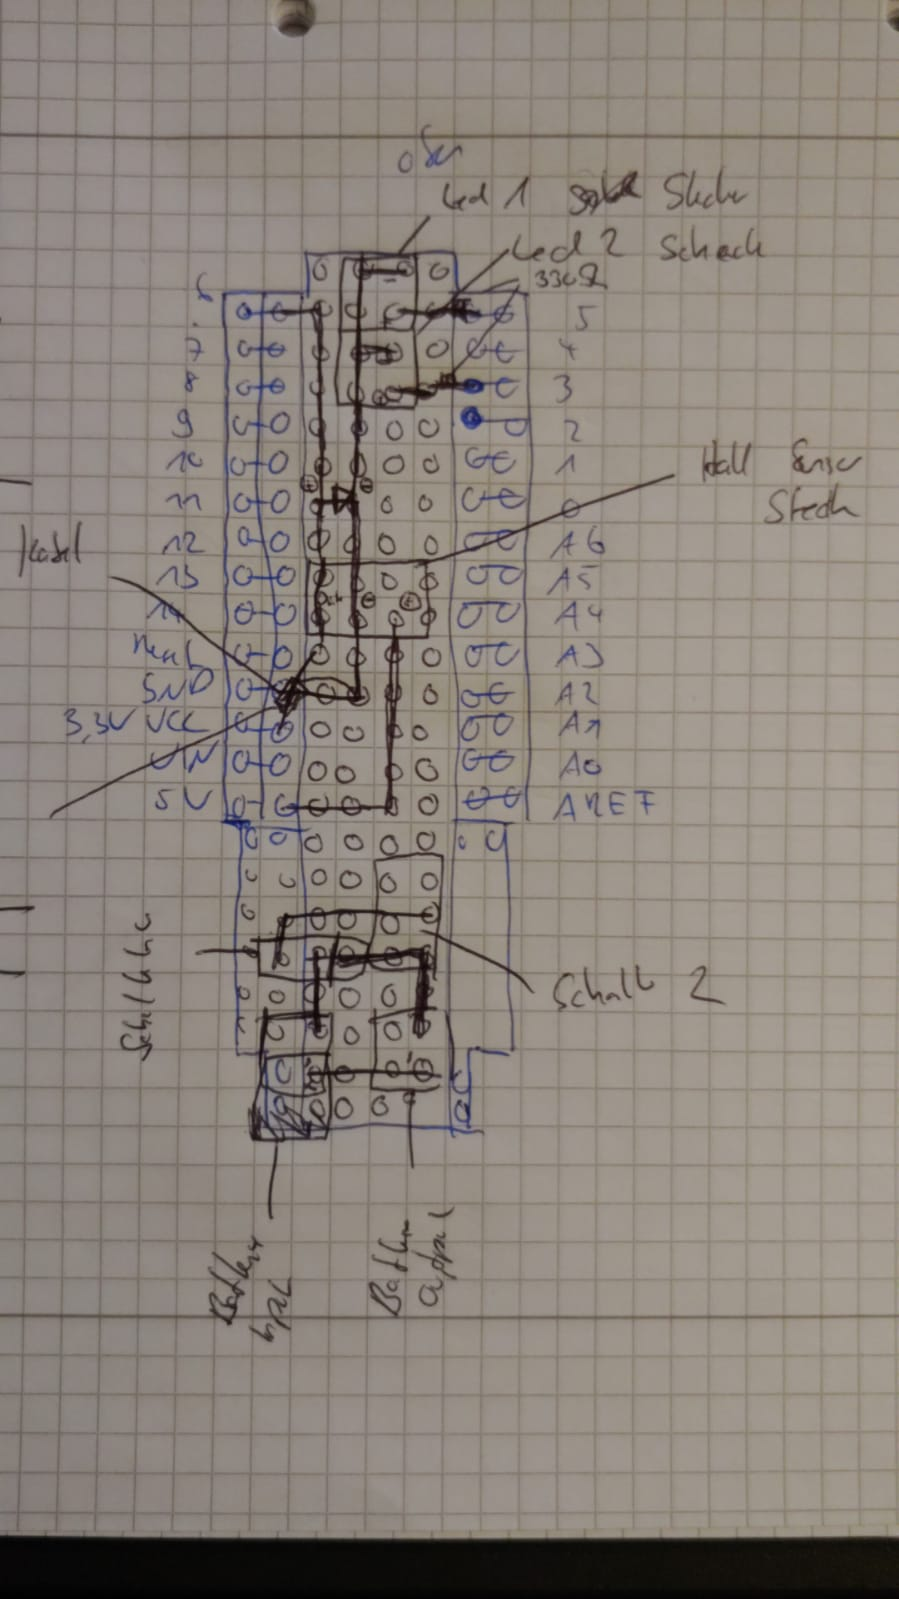
\includegraphics[
    		width=0.5\linewidth,
    		]{imgs/car_wiriring_plan.jpeg}
    		\caption{Konzept für die Fahrzeugplatine}
    		\label{fig-hardware-car-pcb-plan}
    	\end{center}
    \end{figure} 
	\noindent
    Die fertige Platine kann auf den Arduino gesteckt werden, welcher zusammen mit dem Akku, dem $Step-Up Boost-Converter$, dem Sensor und den LEDs in das Auto eingebaut wird. Zusätzlich ermöglicht ein Schalter das einfache an- beziehungsweise ausschalten der Batterie.\\
    Alle Verbindungen zwischen den Komponenten sind mit JST-Steckern realisiert. Dies ermöglicht es, jede Komponente einzeln austauschen, sollte ein Teil defekt sein oder für ein anderes Projekt wiederverwendet werden. Zudem wird so das Zusammensetzen der Fahrzeuge erleichtert, da einige Komponenten wie die LEDs fest in diesen verklebt sind.\\
    Zuletzt wird noch die Konfiguration der Fahrzeuge optimiert. Zuvor haben diese jede Sekunde 1 mal die erfassten Sensordaten gesendet. Da die durchschnittliche Ausführungszeit der \emph{loop}-Funktion bei ca. 100ms liegt, wird dieser Wert auf $250ms$ Sekunden reduziert. Die Fahrzeuge senden häufiger Daten und die Animation bei der Visualisierung werden infolgedessen weicher.
    

\end{document}